\documentclass{article}
\title{Blackjack}
\usepackage[utf8]{inputenc}
\usepackage{hyperref} % for hyperlinks
\usepackage{amssymb}
\usepackage{authblk}
\usepackage{minted}   % for code linting
\usepackage{amsmath}   % big brackets
\usepackage{hyperref}
\usepackage{graphicx} % images
\usepackage{listings, lstautogobble} % gobble

\author{Joshua Ortiga \\
\and
Xin Li \\
\and
Jonathan Le}
\begin{document}
\maketitle

\setlength{\parskip}{\baselineskip}%
\newpage

\section{Background}
\label{sec: Background}

	\subsection{Blackjack Rules}
	\label{sec: Blackjack Rules}

		The rules of Blackjack are simple. Every card in Blackjack (excluding Jokers) are weighed to be worth a certain
		amount of points. All cards from 2-10 are valued at their respective ranks. Face cards (Jack, Queen, and King) 
		are valued at 10 points. Finally, Aces are valued at either 1 or 11 points, and can switch their values at
		any stage of the game. 

		The game starts with the dealer and the player drawing two cards, with the dealer only showing one of their cards.
		In Blackjack, you have the ability to either hit or stand. Hitting will draw you another card, while standing will 
		end your turn, revealing the other dealer's card, and letting the dealer hit until they are at 17 points or higher.

		The goal of the game is to get 21, or closer to 21 points than the dealer without exceeding 21 points. If you have more points than the dealer,
		you win the game. If the points are equal, you draw.
		and finally if you have less points than the dealer, and the dealer's points do not exceed 21, you lose (bust).

		One final aspect of Blackjack to note is that in a real game, money and betting is involved. However, this research paper
		will not cover that aspect of the game. Therefore, surrendering, doubling down and splitting bets will not be considered
		for the scope in the research conducted.

	\subsection{Standard Optimal Strategy}
	\label{sec: Optimal Strategy}

		The optimal strategy when playing a standard game of Blackjack is shown in \hyperlink{fig1}{\textit{Figure 1}}.
		Since betting money is outside the scope of our experiment, any time the chart insists on doubling down, 
		it will instead be assumed to be a hit.
		
		\begin{figure}
			\begin{center}
				\hypertarget{fig1}{}
				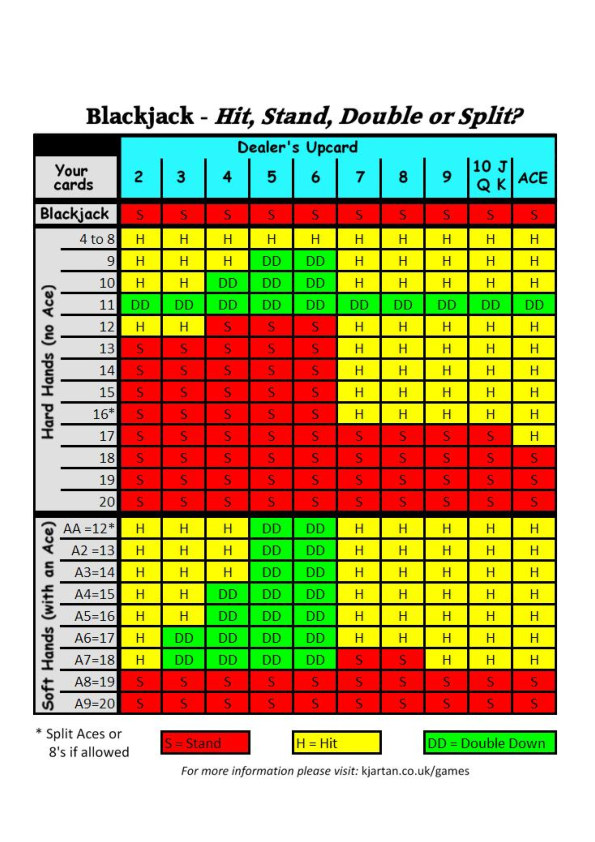
\includegraphics[width=12cm]{blackjack-chart.png}
				\vspace*{-12mm}
				\caption{Standard Blackjack Strategy}
			\end{center}
		\end{figure}


		The x-axes of the charts in the figure describes the dealer's known score. In Blackjack, only one of the dealer's
		initial cards is shown. This means that you can only know some of the dealer's score while it is your turn.
		The player must do their best to play their hand based on what they think the other dealer's card is.
		
		The y-axes of the charts in the figure describes what cards the player has. This is also an important factor
		when the player decides their move because the player needs to play more conservatively if they are at high
		risk of busting (most notably, when the player has more than 11 points).
		
		In \hyperlink{fig1}{\textit{Figure 1}}, there are two sections: \textit{hard hands} and \textit{soft hands}. The player is
		has a \textit{soft hand} when they have an ace in their hand, and can safely hit without busting. This is
		because an Ace can be valued at 1 or 11 throughout the game, so the player's points can effectively "wrap around"
		back to a lower value if they exceed 21 points. This makes hitting far safer, which is why the player should
		be more willing to hit if they do have a \textit{soft hand}.

		In contrast, when a player has no Aces, they have a \textit{hard hand}. The strategy is to play much 
		more conservatively when you have a \textit{hard hand}. This is because if the player goes over 21 points
		without drawing an Ace, they will bust and automatically lose the game.



	\subsection{Hypothetical Rule Changes}
	\label{sec: Hypothetical Rule Changes}

		Blackjack has existed for a long time now, therefore it is a solved game. However, the details of this paper will discuss a hypothetical rule
		change to the game. What if the game was played such that no face cards (Jacks, Queens, and Kings) were not in the decks? How would
		the META (most effective tactic available) of the game change?

	\subsection{Methodology}
	\label{sec: Methodology}
		
		Since testing games of Blackjack manually would take a very long time, our group wrote some Python scripts to simulate
		games of Blackjack in order to gather data for our research. Xin Li wrote the original \href{https://github.com/JDzzz7/Blackjack}{Blackjack simulator} as a summer project.
		Josh Ortiga forked and modified so that it could be used to generate the necessary data and graphs to conduct our research.

		In our Blackjack simulator \href{https://github.com/hosua/blackjack-cs241}{repository}, there are four important scripts
		used to gather our data. All of the scripts automate games of Blackjack and save the data and the graphs of the data to the \textit{data} folder.
		If you are interested, we encourage that you play around with the parameters and generate some data yourself! For more details on how to use the scripts,
		consult the \textit{readme} found in the Github repository.
		\newpage 

		\begin{enumerate}
			\item \textit{optimal\_standard.py} - Simulates standard games of Blackjack and uses the optimal strategy in the figure above.
			\item \textit{unoptimal\_nofaces.py} - Simulates games of Blackjack with the new rules (no face cards) using the same optimal strategy for the standard game of Blackjack.
			\item \textit{optimal\_nofaces.py} - Simulates games of Blackjack with our new optimal strategy given no face cards.
			\item \textit{calc\_busts.py} - Simulates games of Blackjack with no face cards, and records the statistics of the frequency that the dealer busts, as well as which card the dealer 
				had face-up when they busted.
				
		\end{enumerate}

\vspace{0.5cm}
		
\section{Results}
\label{sec: Results}

    \subsection{Optimal Strategy for Vanilla Blackjack}
	\label{Optimal Strategy for Vanilla Blackjack}
		
		{\parindent0pt % remove indent
		Before running simulations for the modified game rules, simulations of standard Blackjack were ran using the optimal strategy depicted in \hyperlink{fig1}{\textit{Figure 1}}.
		
		The Blackjack simulator relies on two dictionaries \textit{hard\_hands} and \textit{soft\_hands} to decide whether or not the player should hit.
		The \textit{hard\_hands} and \textit{soft\_hands} dicts are derived from \hyperlink{fig1}{\textit{Figure 1}}.

		The dict \textit{hard\_hands} is used by the simulator to make a move when the player has no Aces. While the dict
		\textit{soft\_hands} is used by the simulator when the player does have Aces.

		The dict keys are based on the card that the dealer has face up during the player's turn.
		The dict values are pairs consisting of two integers that represent the inclusive range that the player will hit. 
		Note that dict keys 1 and 11 indicate that the dealer has an Ace as their face-up card.
		}

    \begin{minted}{python}
			hard_hands = {
				1: (4,17), # Dealer has ace
				2: (4,12),
				3: (4,12),
				4: (4,11),
				5: (4,11),
				6: (4,11),
				7: (4,16),
				8: (4,16),
				9: (4,16),
				10: (4,16),
				11: (4,17), # Dealer has ace
			}

			soft_hands = {
				1: (12,18), # Dealer has ace
				2: (12,18), 
				3: (12,18), 
				4: (12,18), 
				5: (12,18), 
				6: (12,18), 
				7: (12,17), 
				8: (12,17), 
				9: (12,18), 
				10: (12,18), 
				11: (12,18), # Dealer has ace
			}
        \end{minted}

        \hspace{-0.5cm}After running one million trials of Blackjack games using the standard strategy on a regular deck of cards, the results 
		were as follows:

        \begin{minted}{json}
                {
                    "lose": 475543,
                    "draw": 83990,
                    "win": 440467
                }
        \end{minted}

		Interestingly enough, even when playing with the most optimal strategy, the player is still expected to lose more games than they win.
		This makes sense because house always has edge.

		Now that the data for a standard game of Blackjack has been established, let's run simulations using same strategy on a deck of cards 
		with no faces.
        
		\begin{figure}
			\hypertarget{fig2}{}
			\begin{center}
				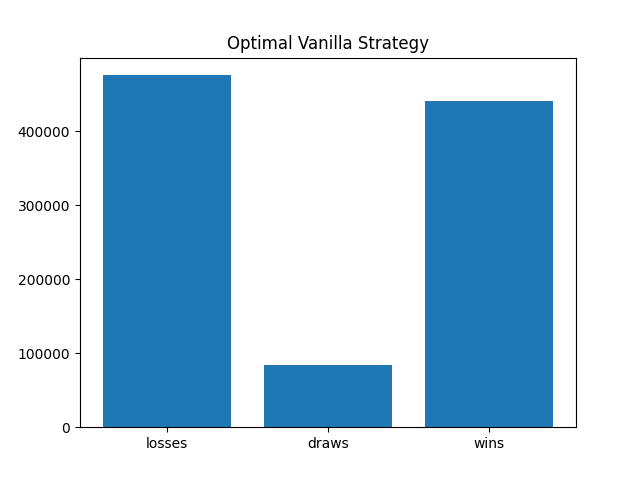
\includegraphics[width=9.5cm]{optimalV.png}
			\end{center}
			\vspace{-10mm}
			\caption{Optimal Vanilla Strategy}
		\end{figure}
		\vspace{2.5cm}

        \hspace{-0.5cm}After running one million trials using the same strategy on the no-face deck, these results were as follows:

        \begin{minted}{json}
                {
                    "lose": 509087,
                    "draw": 82112,
                    "win": 408801
                }
        \end{minted}

		These results are definitely much worse! However, this does line up with expectations. The strategy for vanilla Blackjack shouldn't 
		work well on a deck with no face cards because the strategy is based on the fact that many cards are worth 10 points (10's, Jacks, 
		Queens, and Kings). Since we removed all the face cards from the deck, this is no longer the case. We must now change our strategy to 
		hit more often since the probability of busting is now lower without the face cards.
        
		\begin{figure}
			\hypertarget{fig2}{}
			\begin{center}
				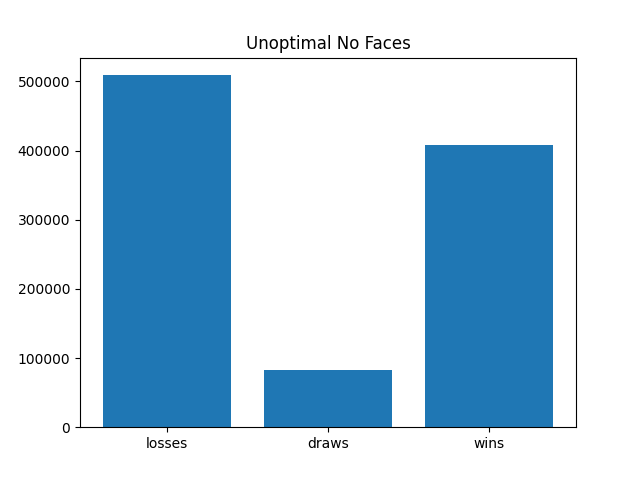
\includegraphics[width=9.5cm]{unoptimalNF.png}
			\end{center}
			\vspace{-10mm}
			\caption{Optimal Vanilla Strategy}
		\end{figure}
        
        \subsection{Modified Strategy For No-Face Blackjack}
		\label{Modified Strategy For No-Face Blackjack}
		\vspace{1cm}
        
		{\parindent0pt % remove indent
			For our \textit{hard\_hands} dict, the lower bounds of our hit ranges will remain unchanged. 

			The only changes that will be made to the \textit{hard\_hands} will be the upper bounds for the keys 2 through 6 inclusive.
			All of their upper bounds will be changed to 16 which will increase how often the simulation will hit. 
			Since there are no face cards, 10 is now the only card valued at 10 points,
			which further implies that the probabilities of the player drawing a card of each value (1 through 11) all now follow an even 
			distribution (when not considering the probabilities of cards that have already been drawn). 

			Since the points of the cards in the deck are evenly distributed with no face cards, hitting when the player is over 11 points 
			is no longer a high risk move as it normally would be in vanilla Blackjack. In vanilla Blackjack, the odds are against you if hit when 
			at 12 or more points because 10's, Jacks, Queens, and Kings are all worth 10 points. Therefore, the odds of drawing a card worth 
			10 points is 4 times more likely than drawing a card of any other value. However, in our deck with no face cards, this is not the case,
			which makes hitting when above 12 points much safer than it normally is, and thus a good motive to change our strategy to fit our new
			deck better.


        
        
		Optimal \textit{hard\_hands} for deck with no faces:
        \begin{minted}{python}
                hard_hands = {
                        1: (4,17), # Dealer has ace
                        2: (4,16),
                        3: (4,16),
                        4: (4,16),
                        5: (4,16),
                        6: (4,16),
                        7: (4,16),
                        8: (4,16),
                        9: (4,16),
                        10: (4,16),
                        11: (4,17), # Dealer has ace
                    }
        \end{minted}

		
		The \textit{soft\_hands} remains unchanged, and will be omitted from this section.

        After running one million trials using our new strategy on the deck with no face cards, the results
		were as follows:

        \begin{minted}{json}
                {
                    "lose": 457774,
                    "draw": 102835,
                    "win": 439391
                }
        \end{minted}

		\begin{figure}
			\hypertarget{fig3}{}
			\begin{center}
				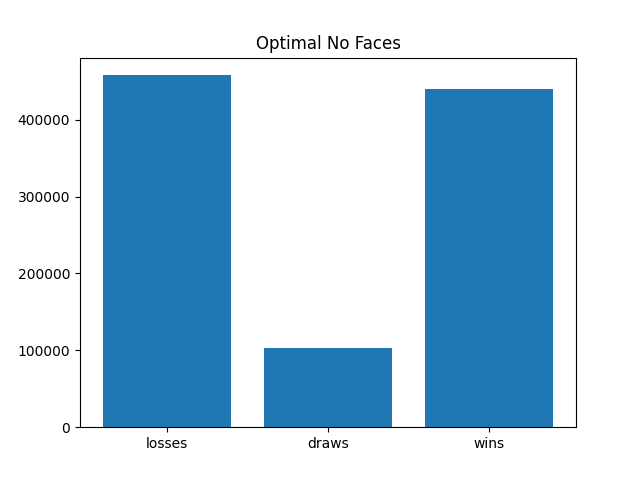
\includegraphics[width=9.5cm]{optimalNF.png}
			\end{center}
		\end{figure}
        
        \subsection{Testing Our New Strategy}
        \label{Testing Our New Strategy}

        Test results after running the standard strategy one million times with the modified no-face deck:

			
		}

        \begin{minted}{json}
                {
                    "lose": 509432,
                    "draw": 81430,
                    "win": 409138,
                    "dealer_bust": {
                        "10": 12127,
                        "2": 20734,
                        "3": 22150,
                        "4": 24376,
                        "5": 26588,
                        "6": 26146,
                        "7": 16392,
                        "8": 14458,
                        "9": 13691,
                        "Ace": 3518,
                        "total": 180180
                    },
                    "dealer_card_freqs": {
                        "10": 100209,
                        "2": 100328,
                        "3": 100232,
                        "4": 99618,
                        "5": 100033,
                        "6": 99812,
                        "7": 100654,
                        "8": 99443,
                        "9": 99926,
                        "Ace": 99745,
                        "total": 1000000
                    }
                }
        \end{minted}

		\begin{figure}
			\hypertarget{fig4}{}
			\begin{center}
				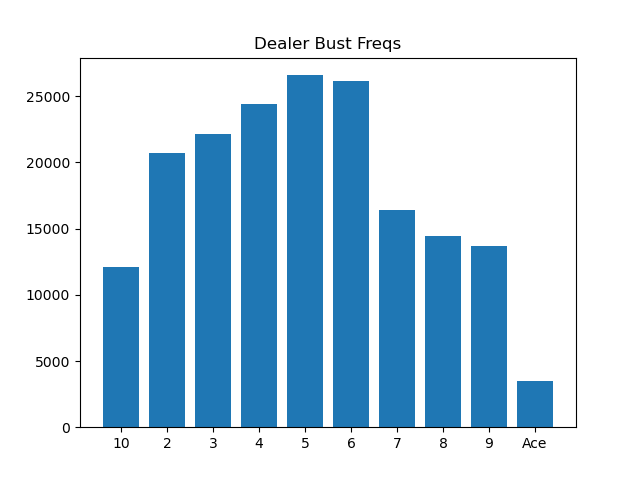
\includegraphics[width=9.5cm]{bustfreq.png}
				\caption{Dealer bust frequencies in 1,000,000 games}
			\end{center}
		\end{figure}

		{\parindent0pt % remove indent
        

        \textbf{Reasoning behind modified hard hands strategy when dealer's face up card is an ace (assuming player total hand is consisting of only two cards):}

        

        In the two cases where the Dealer has an ace, and player doesn't, the chances of the the dealer's face down card being an ace is $\frac{3}{37} = 0.0810810810810811$. Combinations of cards in players hand that add up to 17: (7, 10), (8, 9).

        
        
        Number of cards remaining in deck within the bust threshold (assuming dealer's other card is a card that's 4 or below): $(6 \cdot 4) - 2 = 22$. Number of cards remaining in the deck below the bust threshold: $(4 \cdot 4) - 2 = 14$. If the player stands at 18, the dealer has to bust for the player to win.
        
        
        
        Probability of player busting: $\frac{22}{36}$ = 0.6111

        

        Probability of dealer busting calculated with $\frac{dealer\_bust}{dealer\_card\_freqs}$ Key being starting face up card:
        \begin{itemize}
            \item Ace: $\frac{3518}{99745} = 0.035$
        \end{itemize}

        

        \textbf{Reasoning behind modified hard hands strategy when dealer's face up card is not an ace (assuming player total hand is consisting of only two cards):}

        

        In the rest of the cases where the Dealer doesn't have an ace, and the player doesn't, the chances of the dealer's face down card being an ace is $\frac{4}{37} = 0.1081081081081081$. Combinations of cards in players hand that add up to 16: (6, 10), (7, 9), (8, 8).

        
        
         Number of cards remaining in deck within the bust threshold (assuming dealer's other card is a card that's 4 or below): $(5 \cdot 4) - 2 = 18$. Number of cards remaining in deck below the bust threshold: $(5 \cdot 4) - 2 = 18$. If the player stands at 17, the dealer has to bust for the player to win.
        
        
        
        Probability of player busting: $\frac{18}{36}$ = 0.5

        

		}

        \hspace{-0.5cm}Probability of dealer busting calculated with $\frac{dealer\_bust}{dealer\_card\_freqs}$ Key being starting face up card:
        \begin{itemize}
            \item Two: $\frac{20734}{100328} = 0.21$
            \item Three: $\frac{22150}{100232} = 0.22$
            \item Four: $\frac{24376}{99618} = 0.24$
            \item Five: $\frac{26588}{100033} = 0.27$
            \item Six: $\frac{26146}{99812} = 0.26$
            \item Seven: $\frac{16392}{100654} = 0.16$
            \item Eight: $\frac{14458}{99443} = 0.15$
            \item Nine: $\frac{13691}{99926} = 0.14$
            \item Ten: $\frac{12127}{100209} = 0.12$
        \end{itemize}

        \begin{center}
			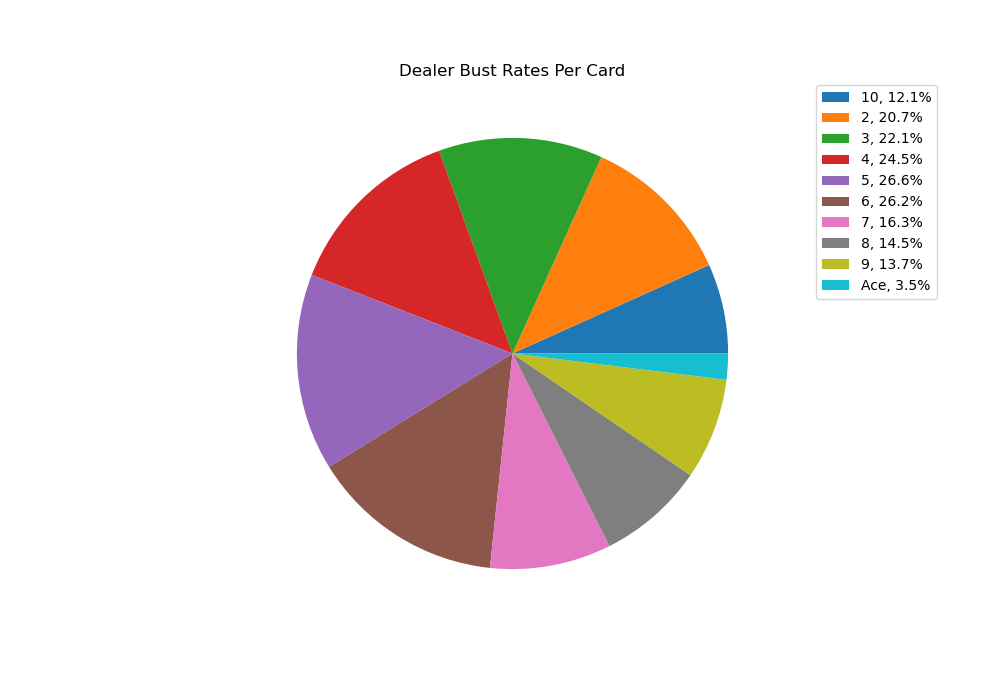
\includegraphics[width=9.5cm]{pie-chart.png}
		\end{center}

        Although the dealer's bust rates is much lower than the player's, if the player were to hit at 18 and above, the chances of busting would be much higher and not ideal. The mean bust rate of the dealer without an ace as a starting card would be: $\frac{sum\_of\_all\_bust\_rates}{9} = 0.197$ 
        This is equivalent to the player having a 20\% chance of winning the game and an even higher chance of getting a tie. 

        \vspace{0.25cm}

        Now if we observe the dealer's bust rates, we can see that the bust rates peak when they have a 5 as a starting face up card. Additionally, the bust rates are much lower from 7-10 (starting card) as compared to 2-6 for the dealer. This is because the dealer has a much higher chance of drawing a card that puts them at 17 or above when the dealer already has a starting face-up card that's more than 6, which lowers their chances of busting since they will not draw as much. The chances of the dealer busting if his starting card is 6 or below is much higher since there is a good chance that they could draw more times and not be at 17 yet. 

        \vspace{0.25cm}

        When the dealer's starting face-up card is an ace, this means it could either be an 11 if it doesn't put them over 21, or a 1 if it does. This explains why the bust rate for when the dealer has an ace is so low at 3.5\%. The amount of times they draw is dependent on their current ace's value, which lowers their bust rate significantly.

        
\section{Summary}
\label{sec: Summary}

        \subsection{Results Synopsis}
	\label{Results Synopsis}

        After running millions of test cases with different player starting hand values, analyzing the test results, and calculating each scenario's probability, we have come to the conclusion that our optimal, no-face Blackjack strategy would be to keep the soft\_hands vanilla strategy and modify the hard\_hands strategy. 

        Using the vanilla blackjack strategy on the modified deck was not ideal due to the missing face cards, and we have been able to produce much higher wins to losses ratio with the strategy that we have developed. 

        \subsection{Table For No-Face Blackjack Strategy}
	\label{Table For No-Face Blackjack Strategy}
         
		\begin{figure}
			\hypertarget{fig5}{}
			\begin{center}
				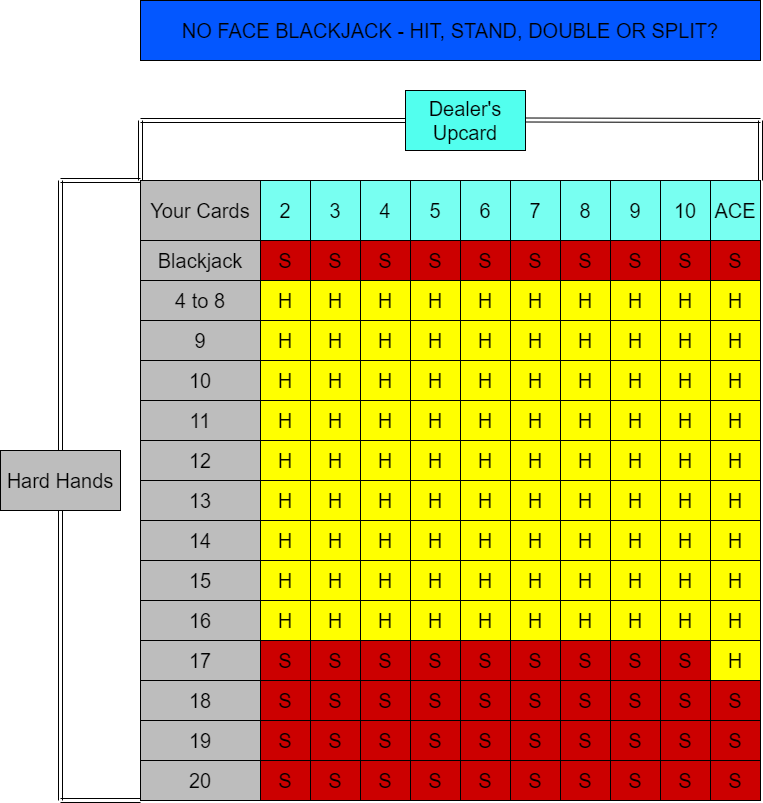
\includegraphics[width=9.5cm]{modified-table-strat.png}
			\end{center}
		\end{figure}

        \subsection{Final Thoughts}
	\label{Final Thoughts}

        As one of the most well known card games used for gambling, this project shows the weight remaining cards can have on a player's decision making and gives us a significantly better insight into the world of Blackjack. 
        
        As shown in our graph's within the background as well as results, removing face cards heavily swings the game towards the house as well as promoting more aggressive strategies in certain scenarios compared to using a normal deck. 
        
        Looking further, high cost cards favor the player's side of the game, as their one advantage over the dealer, being their ability to control when they stand or hit, allows them to maneuver around these cards preventing a bust. This can be seen when observing the chart of the unmodified deck where often the best strategy is aiming for the dealer to bust. When removing the face cards, the chance of busting goes down drastically. This allows the player as well as the dealer to safely hit more often without as much fear of busting. 

        Applying this to other scenarios, we can assume that removing lower cost cards such as from 2-5 will result in the player often just standing as the risk of busting from just one hit is too much, resulting in a very boring match. 
        
        As for potential consequences in the casino industry, many casinos use numerous decks at once to mitigate much of the variation that comes with removing cards from the deck. This, however, doesn't completely nullify these changes. It is unlikely for a single person to completely memorize charts and tables for a given scenario of the deck, but with the rise in augmented reality technology, new programs and software similar to this, in the aspect of giving optimal moves to players, can be used to give players a heavy advantage, assuming players are able to use them without notice.

\section{Works Cited}
\label{sec: Works Cited}
{\parindent0pt % remove indent

	\href{https://github.com/hosua/blackjack-cs241}{Blackjack Simulator}

	\href{https://en.wikipedia.org/wiki/Glossary\_of\_game\_theory}{Glossary of Game Theory}

	\href{https://www.kjartan.co.uk/games/blackjack.htm}{Optimal Strategy Guide}

	\href{https://www.kjartan.co.uk/games/pix/cards/Blackjack%20full%20guide.pdf}{Optimal Strategy Chart}
}
\end{document}
